% Kết quả được trích từ output đã lưu trong notebook; không chạy lại thí nghiệm.
\section{Thực nghiệm và Kết quả}
\label{sec:experiments}

\subsection{Mô tả bộ dữ liệu}
Thực nghiệm so sánh K-means, GMM-EM và DBSCAN trên bộ dữ liệu được notebook
đặt tên là \emph{EV Adoption Prediction}. Output ghi nhận dữ liệu gốc gồm
668.665 dòng và 15 cột. Để giảm chi phí tính toán, notebook lấy mẫu 15.000 dòng
với \texttt{random\_state=42}. Quy trình thu thập, quần thể khảo sát và thời
điểm thu thập không được mô tả; vì vậy, kết quả chỉ phản ánh mẫu thực nghiệm,
chưa đủ cơ sở để khái quát cho người có nhu cầu mua xe điện.

Sau khi loại \texttt{id} và \texttt{Will\_Buy\_EV}, đầu vào gồm 13 đặc trưng.
Dựa trên tên cột, chúng thuộc các nhóm: nhân khẩu học và kinh tế (tuổi,
thu nhập, giới tính); di chuyển và sở hữu phương tiện (quãng đường đi lại
hằng ngày, số xe, loại xe hiện tại); tiếp cận trạm sạc gần nhà và nơi làm
việc; cùng các yếu tố bối cảnh và thái độ (loại đô thị, khả năng sạc tại nhà,
trợ cấp, quan tâm đến môi trường và lo ngại về phạm vi di chuyển).
Đây là cách mô tả theo tên biến; notebook không cung cấp đầy đủ định nghĩa
và quy ước mã hóa của từng cột.

Sáu biến phân loại được mã hóa bằng các đối tượng \texttt{LabelEncoder}
riêng biệt: \texttt{Gender}, \texttt{City\_Type},
\texttt{Current\_Car\_Type}, \texttt{Home\_Charging\_Possible},
\texttt{Subsidy\_Available} và \texttt{Range\_Anxiety\_Level}.
Biến mục tiêu \texttt{Will\_Buy\_EV}, biểu thị nhãn mua xe điện trong bộ
dữ liệu, được mã hóa riêng. Output ghi nhận 12.412 mẫu thuộc lớp mã hóa 0
và 2.588 mẫu thuộc lớp 1. Một biểu đồ chú thích hai lớp là No và Yes,
nhưng ánh xạ của bộ mã hóa không được in ra. Biến mục tiêu và mã định danh
đều bị loại khỏi đầu vào; biến mục tiêu chỉ dùng để đánh giá mức tương đồng
giữa phân hoạch cụm và phân nhóm theo nhãn bằng chỉ số ARI.

\texttt{StandardScaler} chuẩn hóa 13 đặc trưng trước khi khớp cả ba mô hình.
PCA với hai thành phần chính sau đó được áp dụng cho dữ liệu chuẩn hóa
để trực quan hóa. Hai thành phần giữ lại 30.6\% phương sai theo output.
Việc khớp mô hình và tính các chỉ số nội tại sử dụng không gian 13 chiều
đã chuẩn hóa; phép chiếu hai chiều chỉ phục vụ biểu diễn hình ảnh.

\subsection{Cài đặt thực nghiệm}
Notebook sử dụng Python với NumPy và pandas để xử lý dữ liệu;
scikit-learn để tiền xử lý, phân cụm, thực hiện PCA, tìm láng giềng gần nhất
và đánh giá; Matplotlib để vẽ biểu đồ. Mã nguồn hỗ trợ đường dẫn CSV cục bộ
và tải tệp qua Google Colab khi không tìm thấy dữ liệu, nhưng không xác định
môi trường đã tạo ra output lưu sẵn. Phiên bản thư viện và cấu hình phần cứng
không được ghi nhận. Hạt giống ngẫu nhiên của NumPy, bước lấy mẫu và
các mô hình có khai báo tường minh đều được đặt bằng 42.

Với K-means, notebook khảo sát $K=2,\ldots,10$ qua tổng bình phương khoảng
cách trong cụm (inertia) và Silhouette. Output cho biết $K=3$ đạt Silhouette
cao nhất trong phạm vi khảo sát. Tuy nhiên, phép so sánh cuối đặt $K=2$,
với \texttt{n\_init=10} và \texttt{random\_state=42}. Đây là cấu hình
hai cụm được chọn, chưa phải cấu hình được ưu tiên bởi khảo sát Silhouette.
Giới hạn vòng lặp không được khai báo tường minh; thiếu phiên bản thư viện
nên không xác định giá trị mặc định thực tế.

GMM sử dụng \texttt{GaussianMixture} với hai thành phần,
\texttt{covariance\_type='full'}, \texttt{n\_init=5},
\texttt{max\_iter=200} và \texttt{random\_state=42}. Ma trận hiệp phương sai
đầy đủ biểu diễn sự phụ thuộc giữa các đặc trưng trong từng thành phần.
Nhãn cụm cứng được lấy bằng \texttt{predict}, còn \texttt{predict\_proba}
trả về xác suất thuộc từng thành phần. Output ghi nhận hội tụ sau sáu vòng
lặp và tổng log-likelihood trên dữ liệu khớp mô hình là $-112{,}260.46$.
Notebook không cung cấp đường cong log-likelihood qua từng vòng lặp
hoặc phép đo thời gian chạy.

DBSCAN dùng $\varepsilon=2.0$ và \texttt{min\_samples=10}.
Trước khi gán các giá trị này, notebook vẽ đường cong khoảng cách đã sắp
xếp từ \texttt{NearestNeighbors(n\_neighbors=5)}. Bán kính được đặt thủ công
có tham khảo đồ thị, chưa có tìm kiếm tham số chứng minh tính tối ưu.
Số láng giềng khảo sát cũng khác với \texttt{min\_samples} khi phân cụm.

Ba chỉ số được dùng để đánh giá. Silhouette đối chiếu độ gắn kết trong cụm
với mức tách biệt khỏi các cụm khác; giá trị càng lớn càng tốt, còn gần 0
cho thấy phân tách yếu theo tiêu chí này. Davies--Bouldin đo độ phân tán
trong cụm tương đối với khoảng cách giữa các cụm; giá trị càng nhỏ càng tốt.
Chỉ số Rand hiệu chỉnh (Adjusted Rand Index, ARI) so sánh hai phân hoạch
sau khi hiệu chỉnh sự trùng hợp ngẫu nhiên. ARI bằng 1 biểu thị hai phân
hoạch giống nhau; gần 0 biểu thị mức tương đồng gần mốc ngẫu nhiên;
giá trị âm biểu thị mức tương đồng thấp hơn mốc đó. ARI bất biến khi
hoán vị mã cụm và không phải độ chính xác phân loại.

Hàm đánh giá chỉ giữ các quan sát có nhãn cụm $\geq 0$ trước khi tính
\emph{cả ba} chỉ số. K-means và GMM được đánh giá trên toàn bộ 15.000 mẫu,
còn DBSCAN chỉ trên 13.615 mẫu không bị gán là nhiễu. Đây là đánh giá
trên mẫu đã dùng để khớp mô hình; không có tập kiểm tra độc lập hoặc
đánh giá qua nhiều lần lấy mẫu.

\subsection{Kết quả}
Bảng~\ref{tab:ev_metrics} trình bày output so sánh đã lưu, làm tròn đến
bốn chữ số thập phân. Các giá trị sáu chữ số thập phân trong bảng dữ liệu
xuất của notebook nhất quán với kết quả làm tròn này.

\begin{table}[H]
  \centering
  \caption{Kết quả phân cụm trong không gian đặc trưng đã chuẩn hóa.
  DBSCAN loại nhiễu khi tính mọi chỉ số; hai phương pháp còn lại dùng toàn bộ mẫu.}
  \label{tab:ev_metrics}
  \begin{tabular}{lrrr}
    \toprule
    Phương pháp & Silhouette $\uparrow$ & Davies--Bouldin $\downarrow$ & ARI $\uparrow$ \\
    \midrule
    K-means & 0.1649 & 2.2271 & $-0.0057$ \\
    GMM-EM  & 0.1653 & 2.3286 & $-0.0285$ \\
    DBSCAN  & 0.0961 & 2.5860 & $-0.0283$ \\
    \bottomrule
  \end{tabular}
\end{table}

GMM đạt Silhouette cao nhất, nhưng chỉ hơn K-means khoảng 0.0004
(0.165325 so với 0.164939 trong output chi tiết). Cả hai giá trị khá thấp,
chưa cho thấy phân tách mạnh theo chỉ số này. K-means có Davies--Bouldin
thấp hơn, đạt 2.2271 so với 2.3286; hai tiêu chí nội tại vì thế chưa cho
thấy lợi thế nhất quán của GMM. Không có kết quả chạy lặp hay khoảng bất
định để xác nhận độ ổn định của chênh lệch Silhouette.

\begin{figure}[H]
  \centering
  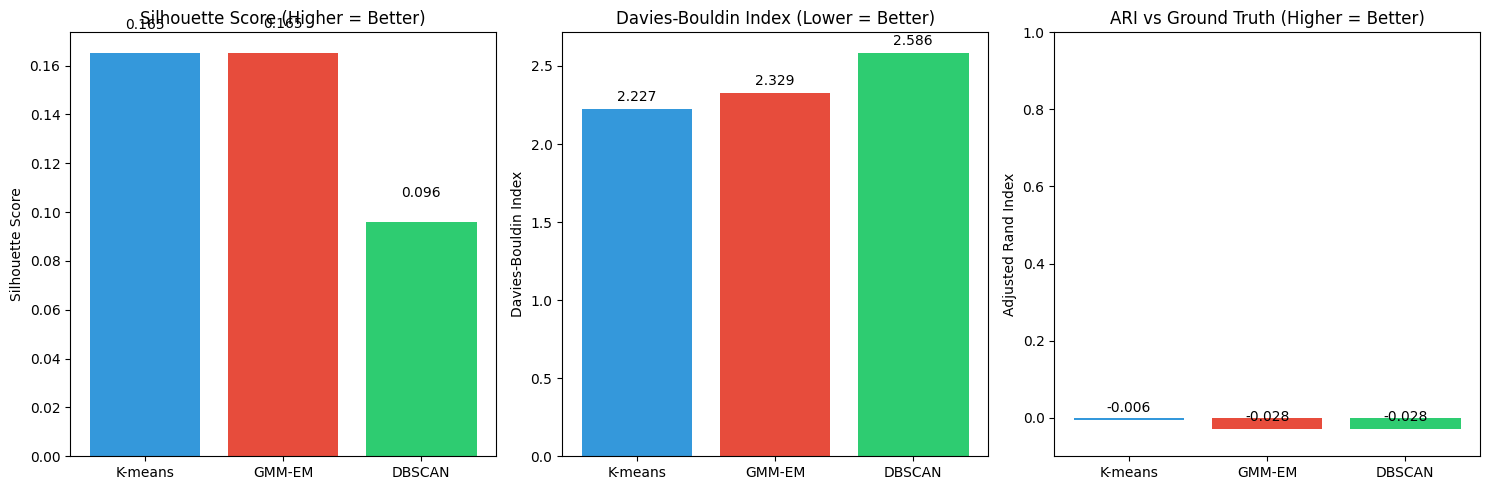
\includegraphics[width=\linewidth]{figures/metrics_comparison.png}
  \caption{So sánh các chỉ số, trích nguyên từ notebook.
  Silhouette và ARI càng cao càng tốt; Davies--Bouldin càng thấp càng tốt.
  Nhãn trên các cột được làm tròn đến ba chữ số thập phân.}
  \label{fig:ev_metrics}
\end{figure}

Hình~\ref{fig:ev_metrics} cho thấy Silhouette của K-means và GMM gần như
bằng nhau; cả hai nhãn làm tròn thành 0.165. Khoảng hiển thị lớn của trục
ARI khiến các giá trị âm khó phân biệt, nên Bảng~\ref{tab:ev_metrics}
phù hợp hơn để đối chiếu chính xác. Cả ba ARI đều âm và gần 0:
các phân hoạch chưa tái hiện được phân nhóm theo nhãn mua xe điện dưới
thước đo này, ngay cả khi xác suất thuộc thành phần cao. Không thể
diễn giải trực tiếp mã cụm thành nhãn dự đoán của \texttt{Will\_Buy\_EV}.

DBSCAN tìm được tám cụm và gán 1.385 quan sát là nhiễu, tương ứng 9.2\%
theo output. Trên các điểm giữ lại, Silhouette đạt 0.0961 và
Davies--Bouldin đạt 2.5860, kém thuận lợi hơn về mặt số học so với hai
phương pháp còn lại. Tuy nhiên, số cụm và tập mẫu đánh giá đều khác nhau;
ngay cả ARI cũng dùng nhãn mục tiêu sau khi lọc nhiễu. Bảng vì vậy phản ánh
từng cấu hình và tập con tương ứng, chưa phải so sánh có kiểm soát trên
cùng tập quan sát. Nhãn nhiễu phụ thuộc tham số mật độ, chưa đủ để kết luận
các bản ghi đó sai hoặc bất thường về mặt thực tiễn.

\begin{figure}[H]
  \centering
  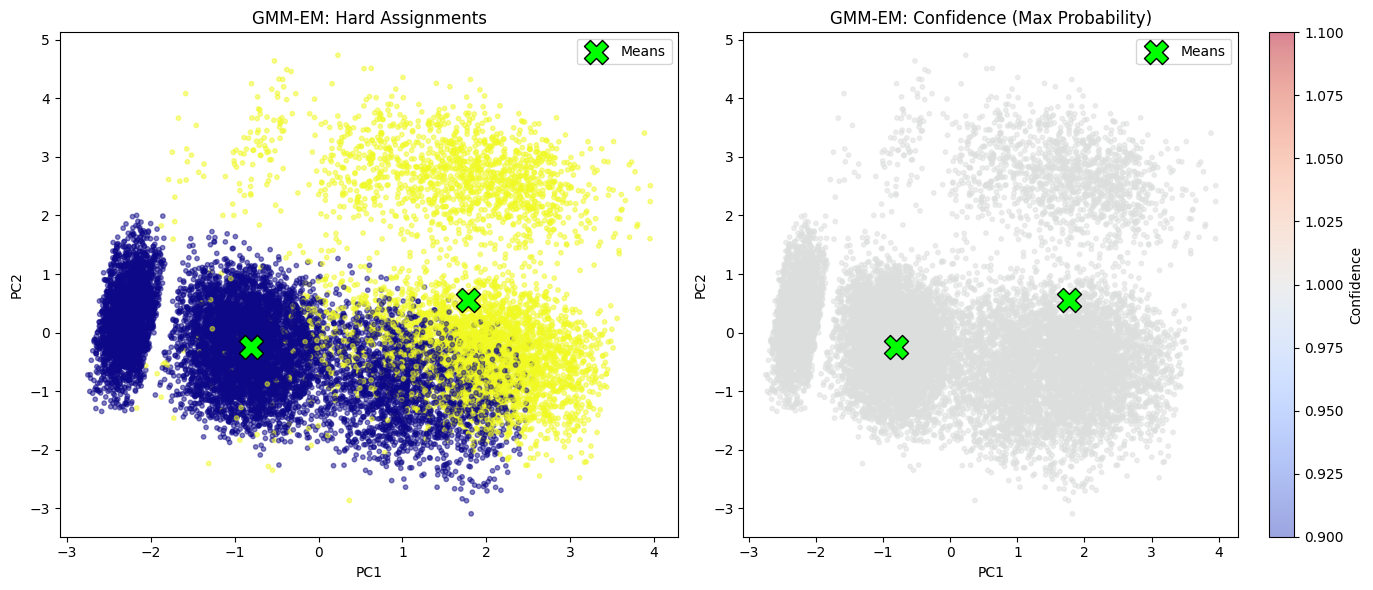
\includegraphics[width=\linewidth]{figures/gmm_clusters.png}
  \caption{Kết quả GMM gốc trên hai thành phần chính: gán cụm cứng (trái)
  và xác suất thuộc thành phần lớn nhất (phải). Dấu chéo xanh lá biểu diễn
  trung bình thành phần sau phép chiếu. PCA giữ lại 30.6\% phương sai.
  Vạch trên 1 của thang màu là hệ quả hiển thị, không phải xác suất hợp lệ.}
  \label{fig:ev_gmm}
\end{figure}

Trong Hình~\ref{fig:ev_gmm}, hai nhóm bên trái có vùng chồng lấn trên phép
chiếu, còn màu bên phải gần như đồng nhất quanh xác suất lớn nhất bằng 1.
Thang màu tự mở rộng từ khoảng 0.9 đến 1.1; vạch trên 1 không biểu thị
xác suất hậu nghiệm hợp lệ. Các xác suất được tính trong không gian
13 chiều, nên chồng lấn trên hình hai chiều không đồng nghĩa với gán cụm
thiếu chắc chắn. Xác suất thuộc thành phần cao cũng chưa chứng minh
các thành phần tương ứng với hành vi mua xe điện hoặc phân khúc có ý nghĩa.

\subsection{Các phát hiện chính}
GMM và K-means có Silhouette gần như bằng nhau tại cấu hình hai thành phần,
trong khi K-means có Davies--Bouldin tốt hơn. Chưa có cơ sở khẳng định GMM
vượt trội đáng kể. DBSCAN tạo phân hoạch nhiều cụm hơn cùng một tập nhiễu,
nhưng các chỉ số nội tại kém thuận lợi hơn chỉ áp dụng cho những điểm giữ
lại tại bán kính và ngưỡng mật độ đã chọn.

Thông tin bổ sung của GMM là vectơ xác suất thuộc thành phần; với hai thành
phần, $\responsibility_{i1}+\responsibility_{i2}=1$. Phần tử lớn nhất
cho biết mức độ mô hình nghiêng về một thành phần khi gán quan sát.
Về nguyên tắc, thông tin này giúp thể hiện trường hợp khó gán cụm,
dù biểu đồ trong lần chạy đã lưu cho thấy rất ít biến thiên.
Đây là xác suất thuộc thành phần ẩn với điều kiện biết đặc trưng và mô hình
đã khớp; không phải xác suất một người sẽ mua xe điện.
Các ARI âm gần 0 càng cho thấy cần phân biệt hai cách diễn giải này.

Hình \texttt{gmm\_uncertainty.png} không được đưa vào báo cáo vì thang màu
diễn giải ngược đại lượng được vẽ. Mã nguồn tính
\[
 u_i=1-2\left|\responsibility_{i1}-0.5\right|.
\]
Với hai thành phần, $u_i=1$ ứng với hai xác suất bằng nhau, tức bất định
gán cụm cao nhất; $u_i=0$ ứng với gán cụm hoàn toàn chắc chắn theo mô hình.
Tuy nhiên, thang màu lại gọi 1 là \emph{certain} (chắc chắn).
Dòng \emph{certainty $>80\%$} kiểm tra $u_i>0.6$, còn dòng
\emph{certainty $<20\%$} kiểm tra $u_i<0.2$; không thể dùng tên các dòng này
để kết luận về mức chắc chắn. Hai output tương ứng, 0.0\% và 100.0\%,
là tỉ lệ đã làm tròn của các điều kiện về bất định trên. Chúng phù hợp với
việc phần lớn quan sát được gán thành phần rõ ràng, chưa cho thấy tình trạng
khó gán cụm xảy ra phổ biến.

Một số giới hạn cần được cân nhắc. Mã hóa phân loại bằng số nguyên tạo ra
thứ tự và khoảng cách có thể không có ý nghĩa thực tiễn; chuẩn hóa không
loại bỏ tác động này. PCA bỏ qua 69.4\% phương sai, hạn chế kết luận từ
hình ảnh. Kết quả chỉ dựa trên một mẫu và một cấu hình cuối có hạt giống
cố định cho mỗi phương pháp, dù K-means và GMM có nhiều lần khởi tạo nội bộ.
Số cụm bằng hai, dạng hiệp phương sai và tham số DBSCAN đều có thể ảnh hưởng
kết quả; khảo sát K-means thực tế ưu tiên ba cụm theo Silhouette.
Notebook cũng không có đánh giá trên tập kiểm tra độc lập, so sánh thời gian
hay phân tích qua nhiều lần chạy. Kết luận về khả năng dự đoán, ưu thế
tính toán và độ ổn định cần được kiểm chứng bằng thí nghiệm bổ sung.
